\section{FPGAs}

FPGA, ou \textit{Field Programmable Gate Arrays}, são dispositivos eletrônicos que são baseados em matrizes de blocos lógicos configuráveis que são conectados via interconexões programáveis \cite{AmdFpga}. Eles podem ser programados e reprogramados para as funcionalidades desejadas.

Sua utilização é necessária em aplicações onde uma implementação em \textit{software} utilizando um microcontrolador não é capaz de cumprir os requisitos de frequência de operação \cite{Sulaiman}.

O que cada bloco lógico possui internamente depende da fabricante e modelo do dispositivo, mas de forma geral possuem pelo menos \textit{Look-Up Tables} (LUTs), que são implementações em hardware de tabelas verdade e elementos de memória, como Flip-Flops \cite{Sato}.

A Figura \ref{fig:FPGAStructure} ilustra a estrutura básica de um FPGA mostrando os blocos lógicos configuráveis, as conexões programáveis.

\begin{figure}[H]
    \centering
    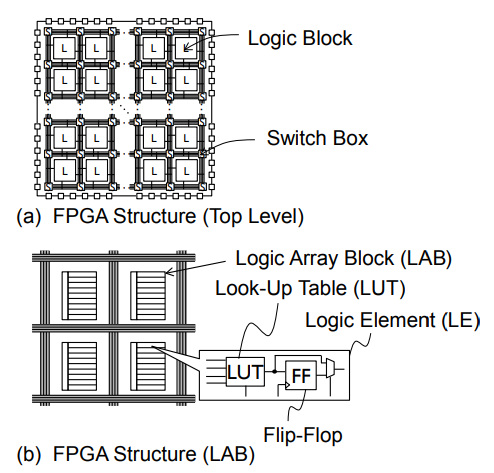
\includegraphics[scale=0.5]{figures/ReferencialTeorico/FPGAStructure.png}
    \caption{Estrutura de um FPGA. Fonte: \cite{Sato}}
    \label{fig:FPGAStructure}
\end{figure}

Os FPGAs são, de forma geral, programados utilizando linguagens de descrição de \textit{hardware} (HDL), sendo VHDL e Verilog as mais utilizadas \cite{Ain}. Essas linguagens, diferentemente de linguagens de programação convencionais onde se escreve uma série de comandos que serão executados de maneira sequencial, descrevem um circuito elétrico que será sintetizado no dispositivo.

A linguagem VHDL é pode ser utilizada para modelar sistemas digitais em diversos níveis de abstração indo do nível de algoritmo ao nível de portas lógicas. A complexidade pode variar do mais simples ao mais complexo \cite{Wunnava}. A Figura \ref{fig:Vhdl} mostra que a linguagem VHDL também pode ser definida como uma combinação de linguagens quando consideramos o nível de abstração.

\begin{figure}[H]
    \centering
    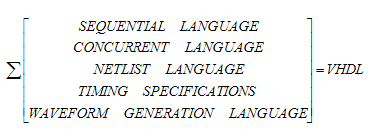
\includegraphics[scale=0.8]{figures/ReferencialTeorico/Vhdl.png}
    \caption{Integração de linguagens que constituem o VHDL. Fonte: \cite{Wunnava}}
    \label{fig:Vhdl}
\end{figure}

% VHDL is a hardware description language employed to model a digital system or digital hardware device at many levels of abstraction, ranging from the algorithmic level to the gate level (Bhasker, 1999a). The complexity of the digital system being modeled could vary from that of a simple gate to a complete digital electronic  system,  or  anything  in  between.  The  digital  system  can  also  be  described  hierarchically.  The VHDL language can also be described as a combination of languages as shown in Figure 1.

A linguagem Verilog permite descrever sistemas digitais desde o nível de portas lógicas ao nível de algoritmo. Também descreve um design do ponto de vista comportamental, de fluxo de dados, estrutural e de atrasos \cite{Bhasker}. Além disso, define sintaxe, semântica e estrutura para realizar simulações, facilitando os testes, em nível de simulação, antes da prototipação e possui simbologia e estrutura parecida com a linguagem C, tornando-se mais familiar para quem for utilizá-la \cite{Wunnava}.
